%% This is file `elsarticle-template-1-num.tex',
%%
%% Copyright 2009 Elsevier Ltd
%%
%% This file is part of the 'Elsarticle Bundle'.
%% ---------------------------------------------
%%
%% It may be distributed under the conditions of the LaTeX Project Public
%% License, either version 1.2 of this license or (at your option) any
%% later version.  The latest version of this license is in
%%    http://www.latex-project.org/lppl.txt
%% and version 1.2 or later is part of all distributions of LaTeX
%% version 1999/12/01 or later.
%%
%% Template article for Elsevier's document class `elsarticle'
%% with numbered style bibliographic references
%%
%% $Id: elsarticle-template-1-num.tex 149 2009-10-08 05:01:15Z rishi $
%% $URL: http://lenova.river-valley.com/svn/elsbst/trunk/elsarticle-template-1-num.tex $
%%
\documentclass[preprint,12pt]{elsarticle}

%% Use the option review to obtain double line spacing
%% \documentclass[preprint,review,12pt]{elsarticle}

%% Use the options 1p,twocolumn; 3p; 3p,twocolumn; 5p; or 5p,twocolumn
%% for a journal layout:
%% \documentclass[final,1p,times]{elsarticle}
%% \documentclass[final,1p,times,twocolumn]{elsarticle}
%% \documentclass[final,3p,times]{elsarticle}
%% \documentclass[final,3p,times,twocolumn]{elsarticle}
%% \documentclass[final,5p,times]{elsarticle}
%% \documentclass[final,5p,times,twocolumn]{elsarticle}

%% The graphicx package provides the includegraphics command.
\usepackage{graphicx}
%% The amssymb package provides various useful mathematical symbols
\usepackage{amssymb}
%% The amsthm package provides extended theorem environments
%% \usepackage{amsthm}

%% The lineno packages adds line numbers. Start line numbering with
%% \begin{linenumbers}, end it with \end{linenumbers}. Or switch it on
%% for the whole article with \linenumbers after \end{frontmatter}.
\usepackage{lineno}

%% natbib.sty is loaded by default. However, natbib options can be
%% provided with \biboptions{...} command. Following options are
%% valid:

%%   round  -  round parentheses are used (default)
%%   square -  square brackets are used   [option]
%%   curly  -  curly braces are used      {option}
%%   angle  -  angle brackets are used    <option>
%%   semicolon  -  multiple citations separated by semi-colon
%%   colon  - same as semicolon, an earlier confusion
%%   comma  -  separated by comma
%%   numbers-  selects numerical citations
%%   super  -  numerical citations as superscripts
%%   sort   -  sorts multiple citations according to order in ref. list
%%   sort&compress   -  like sort, but also compresses numerical citations
%%   compress - compresses without sorting
%%
%% \biboptions{comma,round}

% \biboptions{}

\journal{Journal Name}

\begin{document}

\begin{frontmatter}

%% Title, authors and addresses

\title{Chemical Reaction Path Generation Using State-Space Search Algorithms}

%% use the tnoteref command within \title for footnotes;
%% use the tnotetext command for the associated footnote;
%% use the fnref command within \author or \address for footnotes;
%% use the fntext command for the associated footnote;
%% use the corref command within \author for corresponding author footnotes;
%% use the cortext command for the associated footnote;
%% use the ead command for the email address,
%% and the form \ead[url] for the home page:
%%
%% \title{Title\tnoteref{label1}}
%% \tnotetext[label1]{}
%% \author{Name\corref{cor1}\fnref{label2}}
%% \ead{email address}
%% \ead[url]{home page}
%% \fntext[label2]{}
%% \cortext[cor1]{}
%% \address{Address\fnref{label3}}
%% \fntext[label3]{}


%% use optional labels to link authors explicitly to addresses:
%% \author[label1,label2]{<author name>}
%% \address[label1]{<address>}
%% \address[label2]{<address>}

\author{Sai Srujan Chinta}

\address{Columbia University, New York, NY, United States}

\begin{abstract}
%% Text of abstract
Computer-assisted synthesis design has been in existence since over 40 years now. However, optimum reaction path generators have not been effective in gathering widespread approval by the research community. We propose a completely customizable tool to generate the optimum reaction path given a reactant and a product. Our tool leverages the use of traditional reaction templates combined with the computational complexity afforded by state-space search algorithms. Using reaction templates generated from extensive reaction databases from granted United States patents, out tool automatically generates a tree-like state space structure and searches for the required product intelligently. We report promising results with clearly discernable patterns of behaviour even when the tool fails to find the optimum path. Along with the path, our tool also returns the reaction templates which were used at each step of the reaction, thereby adding more interpretability to the process.
\end{abstract}

\begin{keyword}
A* Search \sep Reaction Path \sep SMARTS
%% keywords here, in the form: keyword \sep keyword

%% MSC codes here, in the form: \MSC code \sep code
%% or \MSC[2008] code \sep code (2000 is the default)

\end{keyword}

\end{frontmatter}

%%
%% Start line numbering here if you want
%%

%% main text
\section{Introduction}
\label{S:1}

Synthesis planning is a task typically performed by highly qualified chemists with decades of experience. In order to assist chemists, retrosynthetic software was developed nearly 40 years ago. Nearly all approaches to automated retrosynthesis involve some use of reaction templates.

In Corey's [1] paper, he proposed a method to extract SMARTS templates from a chemical database of SMILES reaction strings. Specifically, the source of reaction templates is the set of USPTO patents granted between 1976 and 2013, preparsed by Lowe [2]. However, in this data source, contextual information and environmental conditions during each experiment are only sporadically present. Due to the lack of consistent data, all contextual information and environmental conditions (temperature, reagents, catalysts etc.) are dropped and only the reactants and products are considered.  

\section{Methodology}
The overall methodology of this project is shown in Figure \ref{fig:overall_method}. Each individual component is explained in-depth in the following sub-sections.

\begin{figure}[h]
\centering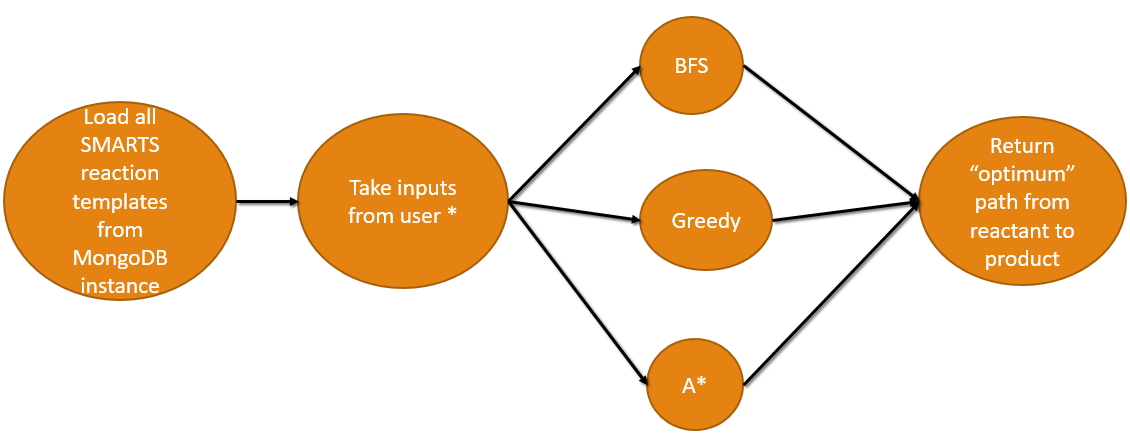
\includegraphics[width=1\linewidth]{methodology.PNG}
\caption{Overall Methodology}
\label{fig:overall_method}
\end{figure}

\subsection{Generating SMARTS templates}

From the 1,122,662 unique reaction SMILES strings, 140,284 unique SMARTS templates are generated [1]. In essence, these reaction SMILES strings are generalised by including wildcard characters which can be replaced by any atom. The process followed for generalising the SMILES strings is as follows:

\begin{enumerate}
\item Identify which atoms have changed from the reactants to the products
\item Generate SMARTS label for each changed atom and make the bond structure and number of Hydrogen atoms explicit
\item Replace the atom-mapped neighbours of the changed atoms with wildcard characters
\end{enumerate}

However, out of the 140,284 unique SMARTS templates generated, the rank versus popularity decays exponentially. This information is clearly encapsulated in Figure \ref{fig:rank_vs_pop}. As we will discuss in the coming sections, our tool allows the end user to customize the number of templates. However, it is in the user's best interest to consider the top few percentage of SMARTS templates because the increased computational complexity does not necessarily yield proportionate results.

\begin{figure}[h]
\centering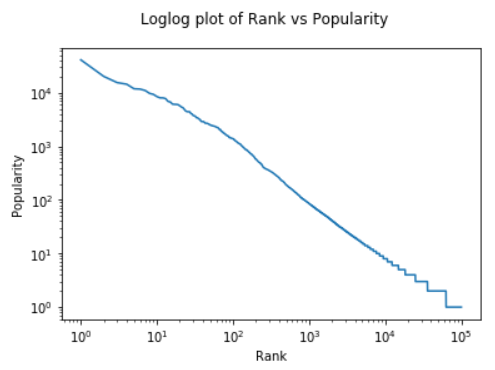
\includegraphics[width=0.6\linewidth]{rank_vs_popularity.png}
\caption{Loglog plot of rank vs popularity of SMARTS templates}
\label{fig:rank_vs_pop}
\end{figure}

\subsection{Inputs from user}
The user first needs to choose among the three state-space search algorithms: Breadth First Search, Greedy Search and A* search.
Inputs common to all the three state-space search algorithms are:
\begin{itemize}
  \item Reactant and Product
  \item Maximum depth of the search tree
  \item Number of SMARTS reaction templates to be used 
\end{itemize}
For both greedy search and A* search, we need a definition of molecular similarity. This definition will be used as a heuristic to gauge the distance between the current molecule and the required product. In this project, we present a choice between radius-2 Morgan circular fingerprints and the default definition of molecular similarity provided by RDKit. 
Additionally, for A* search, we also need the definition of backwards cost. Typically in A* search, backward cost is usually the depth of the current node. However, it is very uncommon for reactions to exceed more than 3 steps. Therefore, using this definition does not make sense because A* search would boil down to BFS with this definition. During our experiments, defining the backward cost as the molecular similarity between the reactant and the current molecule provided the best results in terms of number of nodes expanded and accuracy of results. 

\subsection{Find Optimal Reaction Path}
The final step is to apply the state-space search algorithm with the inputs given by the user. Once the product is found, we return the optimal path, along with all the SMARTS templates at each step of the reaction. If the product is not found before the maximum depth of the search tree (given by the user), then we reverse all the SMARTS templates. Essentially, in each template, the reactants become the products and vice versa. The product is now passed in as the reactant and the reactant is passed as the product. This works because we are still accomplishing the same goal: tracing a chemical route between the reactant and the product. While not all of these reactions may be chemically viable in the opposite direction, this exercise is definitely helpful in gaining valuable insights about the chemical signatures of the reactant and product. In the results section, we explore examples of reactions which initially failed in the forward reaction but returned a path when the templates were inverted and the reactant and product switched. 

\section{Results}
\label{S:2}

In this section, we will discuss a few sample chemical reactions in which our tool was able to find the optimal path and a few reactions where it was unable to find the optimal path. 

\subsection{Found correct optimal path}

Let us first examine a chemical reaction wherein the reactant and product are both aromatic molecules. The reaction that we considered was the conversion from 4-Aminophenol to Benzene, as shown in Figure \ref{fig:aminophenol_to_benzene}.

\begin{figure}[h]
\centering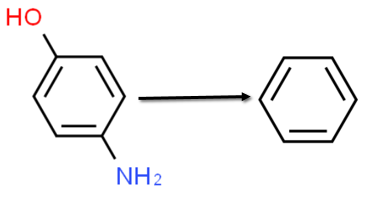
\includegraphics[width=0.4\linewidth]{aminophenol_to_benzene}
\caption{4-Aminophenol to Benzene}
\label{fig:aminophenol_to_benzene}
\end{figure}

Upon feeding in 4-Aminophenol to our tool, it was able to find the optimal path two-step path to Benzene as shown in Figure \ref{fig:aminophenol_to_benzene_path}.

\begin{figure}[h]
\centering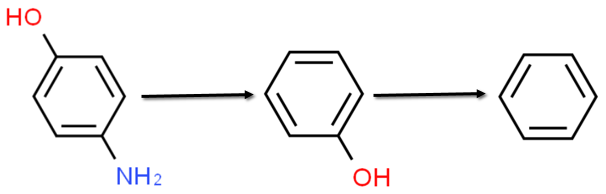
\includegraphics[width=0.6\linewidth]{aminophenol_to_benzene_path}
\caption{4-Aminophenol to Benzene Path}
\label{fig:aminophenol_to_benzene_path}
\end{figure}

Even though our tool does not explicitly return all the molecules (other reactants, reagents, catalysts etc) needed for the above two-step reaction to occur, it does return the SMARTS template corresponding to each of the two steps in the above reaction. In this example, the exact SMARTS templates being used are shown in Figure \ref{fig:smart1} and Figure \ref{fig:smart2}.

\begin{figure}[h]
\centering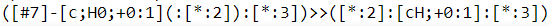
\includegraphics[width=1\linewidth]{templates_aminophenol_to_phenol}
\caption{Template in 4-Aminophenol to Phenol Reaction}
\label{fig:smart1}
\end{figure}

\begin{figure}[h]
\centering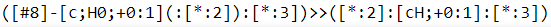
\includegraphics[width=1\linewidth]{templates_phenol_to_benzene}
\caption{Template in Phenol to Benzene Reaction}
\label{fig:smart2}
\end{figure}

]Among aliphatic molecules, we show the example of a standard reaction: hydrolysis of esters to give acids and alcohols. Specifically, we show the hydrolysis of propane butanoate in Figure \ref{fig:butanoate_reaction}

\begin{figure}[h]
\centering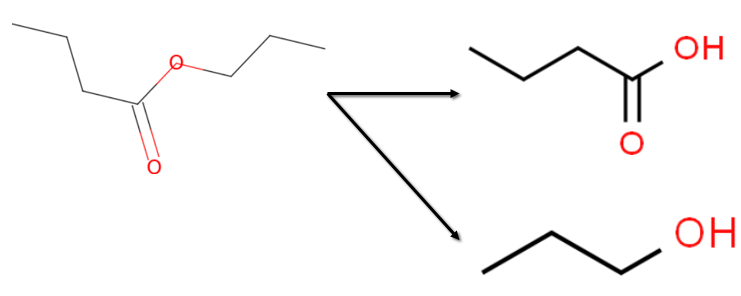
\includegraphics[width=0.6\linewidth]{proponate_to_acid_alcohol}
\caption{Propane Butanoate to Butyric acid and propanol}
\label{fig:butanoate_reaction}
\end{figure}

Our tool also accepts multiple reactants. We show the opposite reaction (Esterification) here as an example. Specifically, the reaction shown in Figure \ref{fig:form_propane_butanoate} is the formation of propane butanoate. 

\begin{figure}[h]
\centering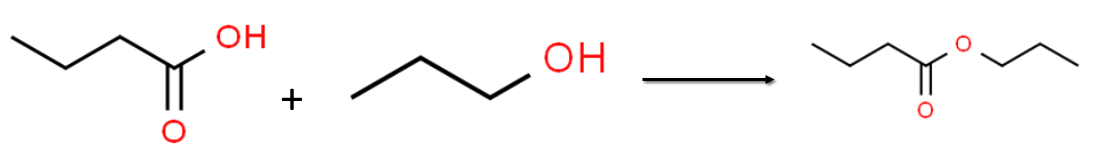
\includegraphics[width=0.8\linewidth]{acid_plus_alcohol_to_ester}
\caption{Butyric acid and propanol to Propane Butanoate}
\label{fig:form_propane_butanoate}
\end{figure}

 \subsection{Did not find correct optimal path}
 
  \begin{figure}[h]
\centering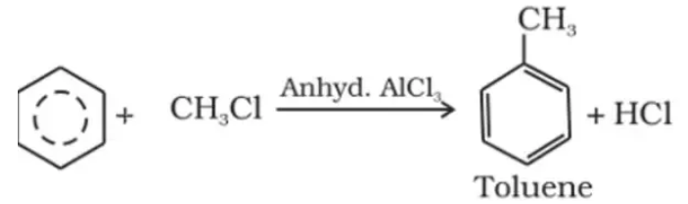
\includegraphics[width=0.8\linewidth]{toulene_from_benzene}
\caption{Toluene from Benzene}
\label{fig:toulene_from_benzene}
\end{figure}

 We will now discuss a couple of examples where our tool was unable to find the correct optimal path. The first example is the creation of Toluene from Benzene as shown in Figure \ref{fig:toulene_from_benzene}. The main reason that this reaction fails is that there is no reaction template which the reactant conforms to which will enable it to add a methane molecule to the benzene ring. However, whenever the forward path fails, we reverse the SMARTS templates and try to find a path. In this case, we were able to go from Toluene to Benzene in a three step reaction. 

 The second example is the creation of aniline from benzoic acid as shown in Figure \ref{fig:aniline_from_benzoic} and Figure \ref{fig:aniline_from_benzoic_part2}. However, the interesting thing about this reaction is that our tool is able to generate the intermediary product. Essentially, our tool is able to reproduce the reaction from Benzoic Acid to Benzamide. However, it fails to finish off the reaction and find Aniline from Benzamide. This is likely because there is no template matching the catalyst (Bromine) in our set of SMARTS reaction templates.
  \begin{figure}[h]
\centering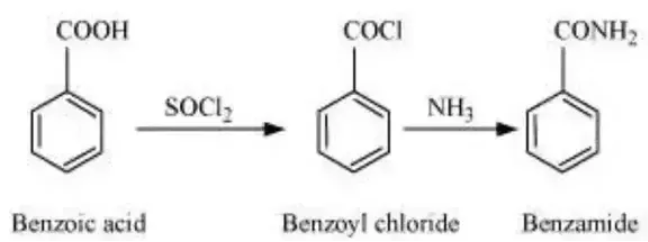
\includegraphics[width=0.8\linewidth]{temp}
\caption{Aniline from Benzoic Acid}
\label{fig:aniline_from_benzoic}
\end{figure}

\begin{figure}[h]
\centering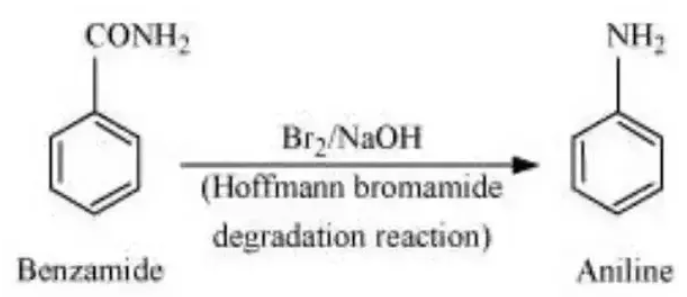
\includegraphics[width=0.8\linewidth]{benzamide_to_aniline}
\caption{Benzamide to Aniline}
\label{fig:aniline_from_benzoic_part2}
\end{figure}

 \subsection{Observations}
 A* search is more efficient than BFS and Greedy search. This is because as the depth of the search tree increases, the number of nodes to expand increases exponentially. Therefore, the order of expansion of nodes is crucial to the smooth functioning of this tool. With BFS, the nodes are expanded (molecules are passed through the given number of SMARTS templates) in the order in which they exist in the search tree. Since this is a brute force approach, it is computationally very expensive (sometimes infeasible) to run BFS on a large number of SMARTS templates and even more so to run it for a decent depth. Within A* search, better results are achieved when molecular similarity is used as a heuristic for backward cost instead of the traditional definition of backwards cost (number of steps taken thus far). The tool tends to perform well for reactions where the product is “simpler” than the reactant chemically, i.e breakdown of chemicals as opposed to creation of complex chemicals. When reactions require a catalyst, the catalyst needs to be added as one of the reactants in the reaction. In general, the tool works better for chained molecules than cyclic molecules.

 

\section{Conclusion}
In this project, we have built a completely customizable chemical reaction path generator for organic chemical reactions. The user can decide how many SMARTS templates to use, which state-space search algorithm to use, specific properties for each search algorithm etc. We leverage the power of search-space algorithms to explore relevant nodes (molecules) first, thereby allowing us to cleverly navigate the search space quickly and efficiently. The results indicate that our tool is successful in finding the optimal path in most cases. Even when it fails to find the path in the forward direction, there is a provision to reverse the templates and find the path from the product to the reactant. In the future, we could add more SMARTS templates at the elementary level to give the resultant path more intuition. Moreover, environmental conditions were not considered while generating the SMARTS templates. Adding this data will add more authenticity to the paths generated by the tool.

\section*{References}

[1] Coley, C. W., Barzilay, R., Jaakkola, T. S., Green, W. H., & Jensen, K. F. (2017). Prediction of organic reaction outcomes using machine learning. ACS central science, 3(5), 434-443.

[2] Lowe, D. M. Extraction of chemical structures and reactions from the literature. Thesis, University of Cambridge, 2012.

%% The Appendices part is started with the command \appendix;
%% appendix sections are then done as normal sections
%% \appendix

%% \section{}
%% \label{}

%% References
%%
%% Following citation commands can be used in the body text:
%% Usage of \cite is as follows:
%%   \cite{key}          ==>>  [#]
%%   \cite[chap. 2]{key} ==>>  [#, chap. 2]
%%   \citet{key}         ==>>  Author [#]

%% References with bibTeX database:

% \bibliographystyle{model1-num-names}

%% New version of the num-names style
%\bibliographystyle{elsarticle-num-names}
%\bibliography{sample.bib}

%% Authors are advised to submit their bibtex database files. They are
%% requested to list a bibtex style file in the manuscript if they do
%% not want to use model1-num-names.bst.

%% References without bibTeX database:

% \begin{thebibliography}{00}

%% \bibitem must have the following form:
%%   \bibitem{key}...
%%

% \bibitem{}

% \end{thebibliography}


\end{document}

%%
%% End of file `elsarticle-template-1-num.tex'.